
\documentclass[11pt]{article}

%%% These are some packages that are useful
\usepackage{circuitikz} %used for circuit diagrams
\usepackage{lastpage} %allows us to determine how many total pages there are
\usepackage{amsfonts, lipsum}
\usepackage{amsmath,amssymb, amscd,amsbsy, amsthm, enumerate}
\usepackage{mdframed, titlesec, setspace,verbatim, multicol}
\usepackage[top=1in, bottom=1in, left=1in, right=1in]{geometry} %sets the margins
\usepackage[unicode]{hyperref} %enhanced references
\usepackage{tikz, xcolor}
\usepackage{fancyhdr} %creates a fancy header for labeling document/name/date 
\usepackage{listings}
\usepackage{xcolor}
\usepackage{vwcol}  
\usepackage{enumitem}
\usepackage{slashed}
\usepackage{subcaption}
\usepackage{ulem}
\usepackage{graphicx}
\newcommand{\ba}{\[\begin{aligned}}
\newcommand{\ea}{\end{aligned}\]}

%%% Page formatting
%\setlength{\headsep}{30pt}
\setlength{\parindent}{25pt}
\setlength{\textheight}{9in}

\title{Money Talks...But All Mine Ever Says is Good-Bye.\\ Using Monte Carlo Methods to Model Financial Transactions.}
\author{Victor Ramirez, Nat Hawkins}
\date{\today}
\graphicspath{{~/Documents/PHY480/PHY480MSU/project4/Report/Figures}}

\begin{document}
\maketitle
\begin{abstract}
	Econophysics is a branch of Physics that has been around since the mid 1990's. It focuses on the use of concepts and practices from multiple areas of study, specifically Statistical Mechanics, and how they can be carried over to observe modern day economical phenomenon. Originally, Physics-based approaches were meant to be used as a secondary approach to provide a secondary explanation for economic occurrences, but soon after extended to observing and predicting new situations. The term was coined due to the large number of papers published by physicists written on topics such as stock market behaviors, wealth distribution modeling, and financial data analysis \cite{wikipedia}. In this project, we created a basic model for financial transactions between two individuals which was ultimately dictated by random number generation in Python. This was then extended to include additional considerations such as savings, interactions with individuals who are close in wealth, and transactions that include some preference for previous interactions between agents. The latter processes are dictated by random number generation and the householder algorithm. We will display results from our analysis as well as draw comparisons to published literature and discuss avenues for future work in Econophysics based on our modeling in this project. 
\end{abstract}
\newpage

\section{Introduction}


\subsection{Motivation}
The allocation of wealth and how income is distributed in society are often used to debate modern economic issues. Most of the wealth tends to be concentrated, as Bernie Sanders would say whilst wagging his index finger, millionaires and billionaires while the rest of the population are left with little. Politicians and economists have been attempting to find ways to reduce the impoverished population and close the income disparity gap. Understanding how this phenomena occurs is an important step in possibly solving this issue.

This phenomena was notably studied by Vilfredo Pareto, an Italian economist and engineer who studied how a system of bodies reached equilibrium in the 1870's. Pareto would expand this study into economics and develop insights on how income distribution equilibrates. The result would become known as the Pareto Distribution, a power law probability distribution that has applications in many fields including physics. Namely, the Pareto Distribution can also be used to describe the sizes of meteors and the Bose-Einstein Codensate. The Pareto Distribution is also an integral building block to the growing field of Econophysics.  \cite{pareto}

\subsection{Mathematics} \label{math}
One of the reasons we chose to pursue this avenue of study in this project is the computational simplicity of this type of modeling. The equations that dictate the behavior of the agents during their various transactions are relatively simple and can be programmed into Python in just a few lines of code. Despite the brevity of the code, the insights we developed were profound enough to dedicate an entire section to it.

The base for our modeling exercise is the modeling of Pareto's work \cite{pareto}. From Pareto’s work (V. Pareto, 1897) it is known from empirical studies that the higher end of the distribution of money follows a distribution of wealth, $w_m$ given as
\ba
w_m \propto m^{-1-\alpha}
\ea
where me denotes the amount of money in question and $\alpha \in [1,2]$. This equations states that the distribution of wealth within a "society" should follow an exponential relationship. 

In all of these financial transactions, two agents selected by index, $i$ and $j$, have some amount of money prior to the transaction given as $m_i$ and $m_j$ respectively. We make the assumption that no agent can go in to debt ($m>0$ for all transactions). This removes the possibility of negative values of wealth being introduced into society. While this is unrealistic, we can relate this to statistical mechanics concepts such as ideal gas behavior.

The transaction at a base level then involves the generation of a random number $\epsilon$ from 0 to 1, which is generated using the random.uniform library in Python. The amount of money that each agent has after the transaction is given as
\ba
m_i &\rightarrow m_i'\\
m_j &\rightarrow m_j'\\
m_i' &= \epsilon (m_i+m_j)\\
m_j' &= (1-\epsilon)(m_i+m_j)
\ea
The random number generation predicts the percentage of the total money between the two agents each person ends up with after the transaction has occurred. In a typical sense, we would expect that one person is the "seller" and gets some amount of money and the other is the "buyer" who gives money to the seller. Here, we describe this interaction as a mutual exchange of goods/services, so instead of one person winning and the other losing, there is an exchange for mutual benefit. From this and the results from Patriarca \cite{patriarca}, the final distribution of the wealth should be in the form of 
\ba
w_m=\beta \exp{(-\beta m)}
\ea

When we included savings into the equation (pun intended), the only difference is that some amount of money is being withheld from the transaction. Now, instead of the total amount of money $m_+m_j$ being exchanged is $(1-\lambda)(m_i+m_j)$. Now the amount of money that each individual has after the transaction has occurred is
\ba
m_i' &= \lambda m_i+\epsilon(1-\lambda)(m_i+m_j)\\
m_j' &= \lambda m_j+(1-\epsilon)(1-\lambda)(m_i+m_j)\\
\ea
which can be written more conveniently in the form
\ba
m_i'&=m_i+\delta m\\
m_j'&=m_j-\delta m\\
\delta m &=(1-\lambda)(\epsilon m_j-(1-\epsilon)m_i)
\ea
Here, $\epsilon$ is still a randomly generated uniform number, but $\lambda$ is now a user set input denoting the amount of money that is being withheld during the transaction. Here, we expect the results to follow a normal (bell-curve) distribution as discovered by Patriarca et al. \cite{patriarca}. 

The two other cases we considered were more complex in meta terms, but computationally no different. The first of these two cases is the consideration of "nearest neighbor" interactions. Here we say that the probability for two agents to interact scales as the absolute value of the difference between wealths
\ba
p \propto |m_i-m_j|^{-\alpha}
\ea
where $\alpha$ is a parameter that we can toggle. This says that the closer two agents are in wealth, the more likely they are to have a financial event. This is then compared to another random number generated within the transaction loops. If the probability value is larger than the uniform random number we generate within the loop, then the transaction occurs using the same functionality as the basic transaction model where some amount, $\epsilon$, of the total money is exchanged. This is in accordance with Householders algorithm. If the agents have the exact same wealth, then the probability of interaction is said to have occurred definitively (p=1). This can be amended to also model simulations that include savings, but the outcome is still the same as dictated by the literature as following $w_m \propto m^{-1-\alpha}$ \cite{goswami}. The larger the value of $\alpha$, the closer agents have to be in wealth for there to be a significant probability of transactions occurring.

The second of these interactions we accounted for previous interactions. The probability now scales as 
\ba
p_{ij} \propto \vert m_i-m_j\vert^{-\alpha}\left(c_{ij}+1\right)^{\gamma}
\ea
where $c_{ij}$ denotes the number of previous interactions between agents $i$ and $j$ and $\gamma$ is another user set parameter with a similar meaning to $\alpha$ in the previous case. The larger the value of $\gamma$, the more the probability is weighted by previous interactions.

The final product of these two cases will be a comparison to the famous "Pareto Tails" found by Goswami and Sen \cite{goswami}. 

\section{Equilibrium} 
In the literature, there is a lot of discussion about the equilibrium state or steady state distribution. This is the point where additional financial transactions do not yield a change in the distribution of the wealth of the society. Another way to think of this is that, like a statistical mechanical system, the society has reached its more probable distribution.

The literature discusses many ways of deciding when equilibrium is reached. These range from looking at when the standard deviation goes to a steady states value (net fluctuation about the mean value) \cite{patriarca} or looking at when the differences in the distributions goes to zero by comparing datasets \cite{goswami}. We made an assumption that the number of transactions that we had the society performed was larger than the number of transactions required for the system to reach whatever equilibrium condition could have been set. This was for multiple reasons. For one, it was simpler to implement computationally (a while loop that terminates after some set number of transactions allowing for easy plotting), and also it reduced the likelihood of error in improperly determining an equilibrium condition. Since beyond equilibrium, the distributions do not change, then additional transactions beyond the equilibrium condition are assumed to have no affect on our results. It also reduces CPU time and load because it eliminates the need to check some calculated value against previous calculations through each iteration. The goal is always elegant and fast programming, so this measure was taken accordingly. 

Therefore, we still are enacting an equilibrium condition: equilibrium is achieved in some number of transactions that we assume is less than the number of transactions we dictate the society conduct. Further work could be done in providing a more analytic expression in accordance to the literature.

\section{Basic Transactions} \label{basic}

The first step of this project is to model basic financial transactions made by agents. We assume the following:
\begin{itemize}
	\item Each agent starts off with the same nonzero amount of wealth $m_{0}$
	\item The total wealth within the society is relatively conserved \footnote{See \ref{conservation}}
	\item No agent gets into debt, i.e. no negative wealths
\end{itemize}

We make the agents by creating an array of some user set size and assigning every cell in the array to some numerical value that is equal to the amount of money that that "person" (index) has. This way, we can keep track of the individual via the indices and the wealth based on the values of the cells.

In each iteration, a random number generator chooses two agents $A_{i}$ and $A_{j}$ assigned by indices $i$ and $j$ to trade. $A_{i}$ then trades a randomly generated portion $\epsilon$ of its wealth to $A_{j}$. We repeat these iterations $10^{6}-10^{7}$ times and show that the wealth distribution follows the Pareto Distribution discussed in \ref{math}. Most of the wealth is concentrated among a few agents, while the most agents are left with a small amount of the wealth. This is consistent with real income distributions. A summary of some of these results are offered in Figure \ref{exp}.

\begin{figure*}[h!]
	\centering
	\begin{subfigure}{0.3\textwidth}
		\centering
		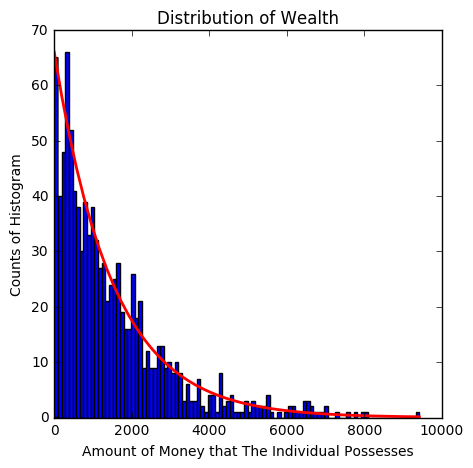
\includegraphics[height=4cm]{exp_1.png}
	\end{subfigure}%
	~ 
	\begin{subfigure}{0.3\textwidth}
		\centering
		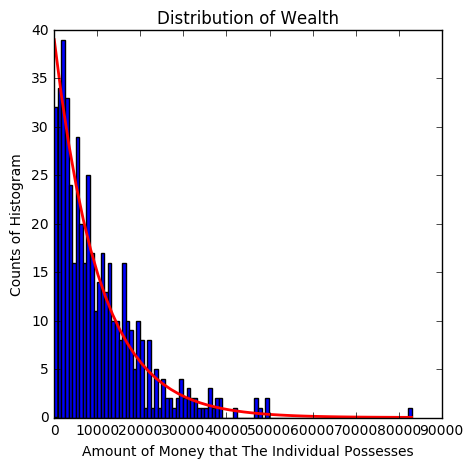
\includegraphics[height=4cm]{exp_2.png}
	\end{subfigure}       
	~ 
	\begin{subfigure}{0.3\textwidth}
		\centering
		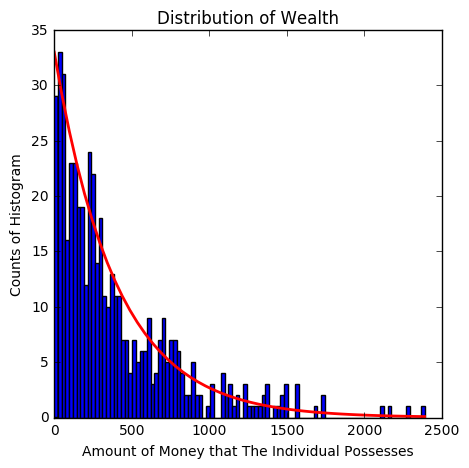
\includegraphics[height=4cm]{exp_3.png}
	\end{subfigure}
	\caption{The wealth distribution of three trials. The bars are counts for each wealth "bin", while the fit is an exponential decay. These are for various amounts of agents with different amounts of starting wealth. The fit verifies that our model obeys the Pareto Efficiency Law.} 
	\label{exp}
\end{figure*}


\section{Introduction of Savings}

We expanded this model to introduce savings. We use a predetermined parameter $\lambda$ that an agent saves before each transaction, described in \ref{math}. Our result for the basic model was made with $\lambda$ = 0. We ran trials for $\lambda$ = 0.25, 0.5, 0.9 at $N$ = 500, 1000 agents. The trials for $N$ = 500 and 1000 were nearly identical; the main difference was that higher $N$ values take longer to equilibrate and form a sharper normal distribution for higher savings values. Because the transaction value was fixed, our final result for $N$ = 500 is closer to equilibrium. The trials for changing $\lambda$ show that the resulting income distribution shifts from a Pareto Distribution to more of a Gaussian Distribution as $\lambda$ is increased. This agrees with the results of Patriarca et al. \cite{patriarca}. The summary of results for our modeling is shown in Figure \ref{gauss}.

\begin{figure*}[h!]
	\begin{subfigure}{0.3\textwidth}
		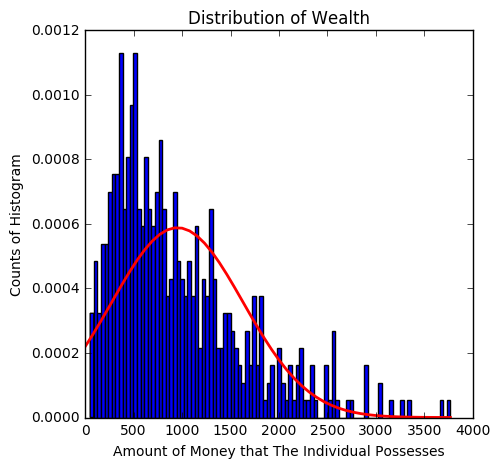
\includegraphics[height = 4cm]{gauss_1_500.png}
		\caption{$\lambda$ = 0.25, N = 500}
	\end{subfigure}
	~
	\begin{subfigure}{0.3\textwidth}
		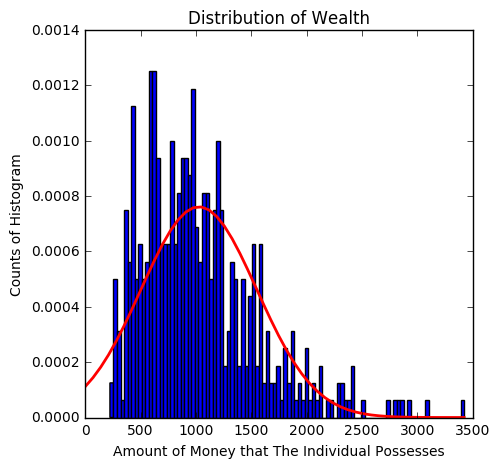
\includegraphics[height = 4cm]{gauss_2_500.png}
		\caption{$\lambda$ = 0.5, N = 500}
	\end{subfigure}
	~
	\begin{subfigure}{0.3\textwidth}
		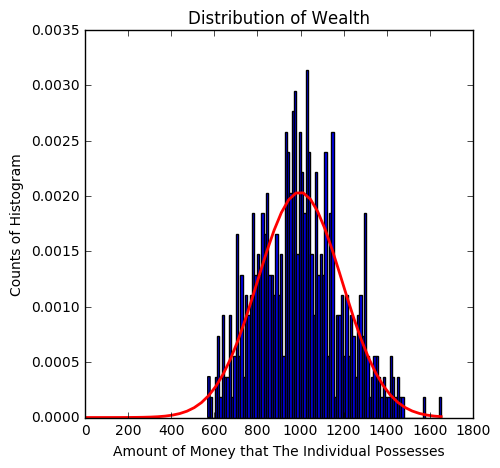
\includegraphics[height = 4cm]{gauss_3_500.png}
		\caption{$\lambda$ = 0.9, N = 500}
	\end{subfigure}
	\caption{The income distributions of varying $\lambda$ at N = 500. The income distribution resembles more of a Gaussian distribution at higher $\lambda$.}
	\label{gauss}
\end{figure*}

\section{More Complex Problems}
\subsection{Nearest Neighbor}
The basic framework of the nearest neighbor interaction is outlined in Section \ref{math}. 

For this section, we had to redefine how we initialize agents. Typically, we would make an array with all of the same values (everyone starts with the same amount of money). In this scenario, if everyone started with the same amount of money, then the probability for interactions would always be equal to 1 (since we defined that in instances of exactly the same wealth transactions occur definitively), and nothing interesting would occur. So, for these advanced trials, we ran this using a uniform distribution to give everyone some amount of money within a given range. 

We first begin by looking at the $\alpha$=0 case. Here, we say that the probability of transactions occurring is equal to 1, so the transactions occur definitively as discussed earlier. 

The trial for our $\alpha=0$ case is shown in Figure \ref{alpha0}. For the case where $\alpha$=0, we get that the probability for interactions is 1, which means that all agents engage in transactions. We ran this trial for only $10^5$ transactions due to computational load, so we do not see the same sort of peak in the exponential decay of the plot. We do still see that along the lines of this unit test, we still get the earlier produced results where our distributions follow the exponential $w_m \propto m^{-1-\alpha}$. 

\begin{figure}[h!]
	\centering
	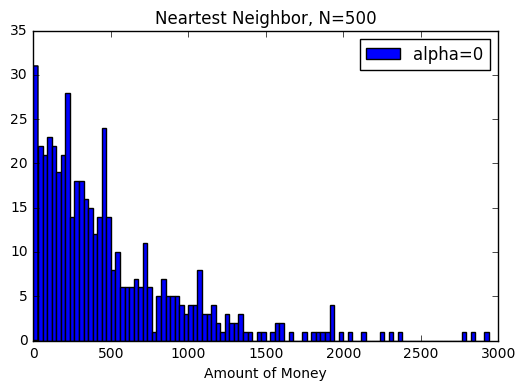
\includegraphics[height=4cm]{nearest_500_0.png}
	\caption{Nearest neighbor case for $\alpha$=0. We can see that we still get the expected exponential distribution of wealth that we got in \ref{basic}. This served as a unit test to ensure that our program would reproduce previously achieved results given the proper inputs.}
	\label{alpha0}
\end{figure}

Now, if we run this with $\alpha=0.5,1.0,1.5,2.0$, we get similar distributions for small $\alpha$. As we increase the value of $\alpha$, the likelihood of transactions begins to get smaller and smaller. This means that we gradually lose our exponential distribution and it becomes slightly more "flat". This is because only people who are extremely close in wealth have any significant probability of interacting. This is emphasized in Figure \ref{bigalpha}. The distributions are shown in figure \ref{near500} both with and without savings. The distributions looks somewhat different in terms of scaling, but overall we see the same general trend. 

\begin{figure}
	\centering
	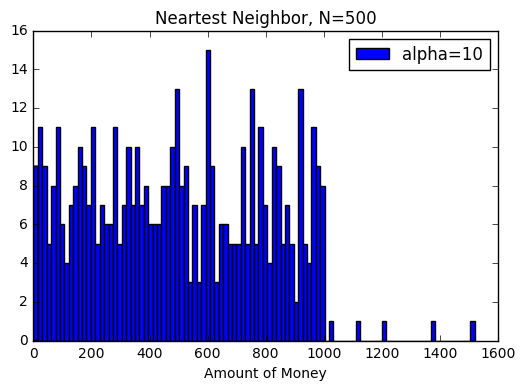
\includegraphics[height=4cm]{nearest_500_10.png}
	\caption{The nearest neighbor interaction with $\alpha$=10. At large values of $\alpha$, the distribution of wealth continues to become "flatter" and closer to the initial distribution of wealth due to the low probability of interactions for people of different wealths.}
	\label{bigalpha}
\end{figure}

\begin{figure*}[h!]
	\centering
	\begin{subfigure}{0.45\linewidth}
		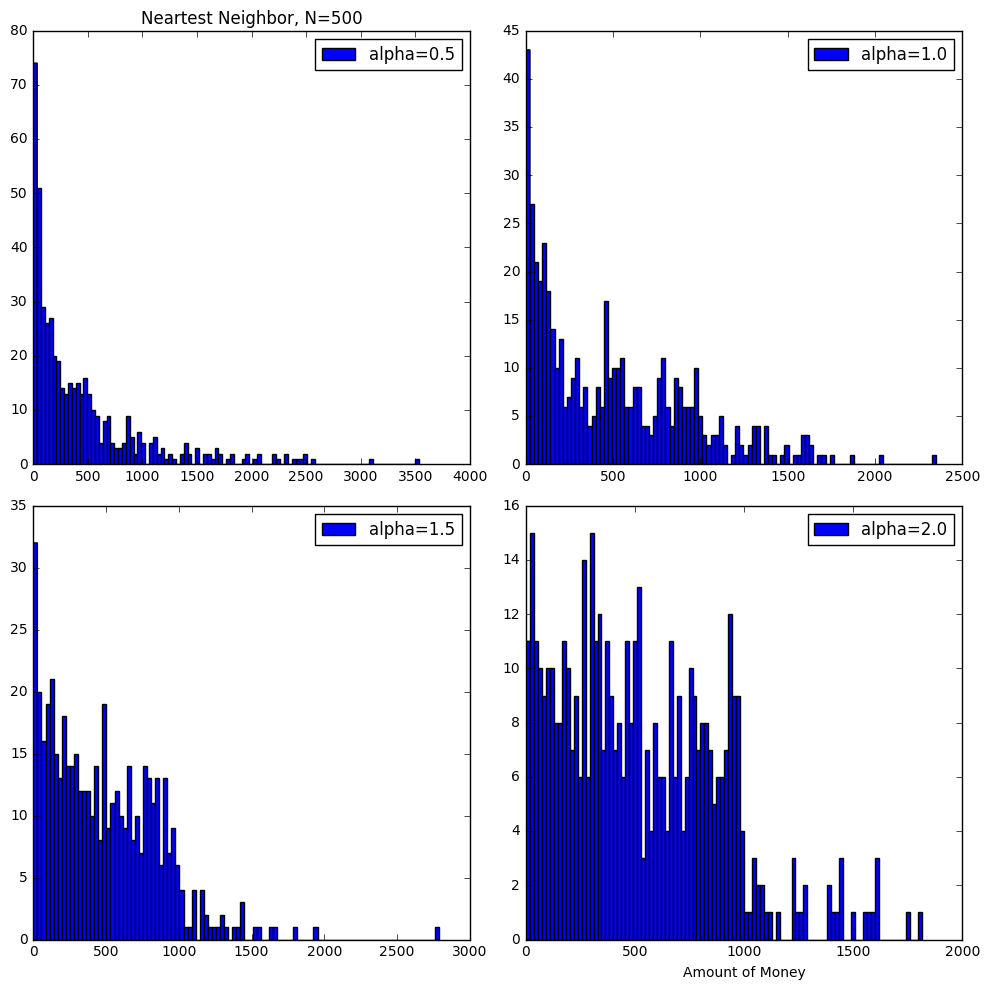
\includegraphics[height=5cm]{nearest_500_subplots.png}
		\caption{Subplots for the nearest neighbor interactions as dictated by our algorithm. The values of alpha are listed on the plots. This is for N=500 and no savings.}
	\end{subfigure}
	~
	\begin{subfigure}{0.45\linewidth}
		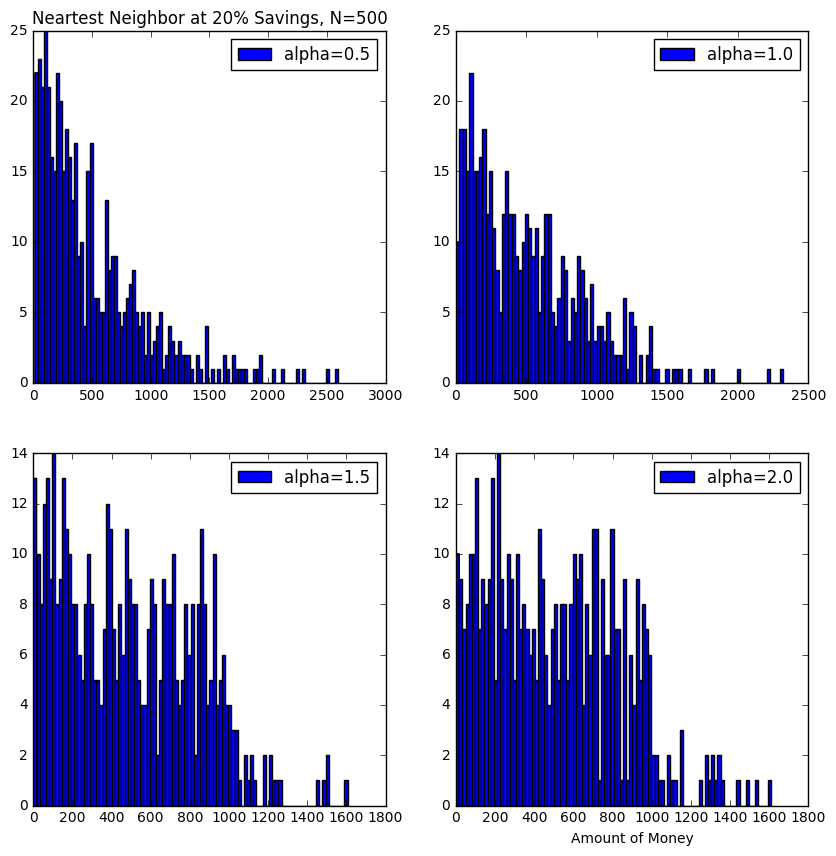
\includegraphics[height=5cm]{nearest_savings_20_500.png}
		\caption{Subplots for the nearest neighbor interactions as dictated by our algorithm. The values of alpha are listed on the plots. This is for N=500 at 20\% savings.}
	\end{subfigure}
	\caption{The above plots show the nearest neighbor wealth distribution for N=500 with and without savings.}
	\label{near500}
\end{figure*}

These results follow our expectations of the literature \cite{goswami}. The more impressive results come with the recreation of the Pareto tails. See Section \ref{previous}. From our wealth distribution data, we were also able to recreate the log plots seen in \cite{goswami}.

\begin{figure}
	\centering
	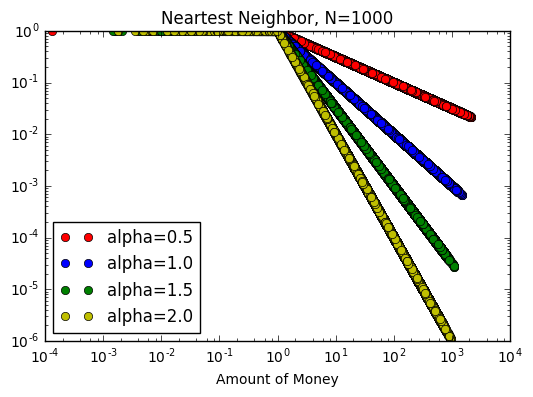
\includegraphics[height=4cm]{log_nearest.png}
	\caption{Recreation of log plots from Goswami and Sen. Verifies exponential distributions of wealth in society as dictated by $w_m \propto m^{-1-\alpha}$.}
	\label{logs}
\end{figure}

\subsection{Previous Interactions with Nearest Neighbors} \label{previous}
The last expansion to this program is to account for previous transactions made by agents. To model more realistic transactions, we added an additional parameter that makes agents more likely to trade with those similar in wealth and have a history of transactions together. We introduce the parameter $\gamma$ which dictates how strongly these factors affect the likelihood of two agents trading. The higher the $\gamma$, the more an agent "values" past transactions and vicinity and wealth, making it more likely to trade with another agent that shares those attributes. The probability to make a transaction is discussed in the last section of \ref{math}. An analogous model was created by Goswami and Sen \cite{goswami} and we used their results as a benchmark for our results. 

We created a log-log plot the probability P(m) as a function of the money m. We saw that our results matched that of the literature \cite{goswami}. In particular, the "tails" of the distribution matched the expected behavior: The higher the $\gamma$, the sharper the drop in P(m) as a function of m. In other words, the income disparity becomes more pronounced as $\gamma$ is increased. These plots are shown in Figure \ref{Pareto}.

\begin{figure*}[!ht]
	\begin{subfigure}{0.5\textwidth}
		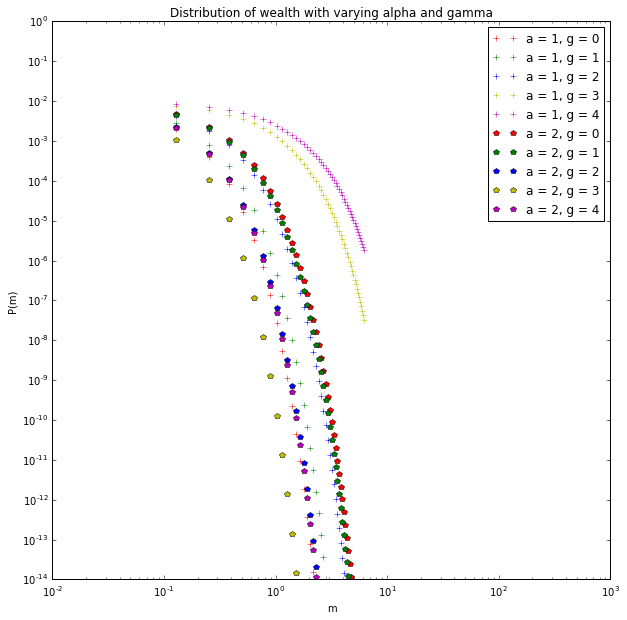
\includegraphics[height = 5.5cm]{Pareto_Distribution.png}
		\caption{Probability P(m) as a function of the money m for the nearest neighbor and past transactions model.}
	\end{subfigure}
	~
	\begin{subfigure}{0.5\textwidth}
		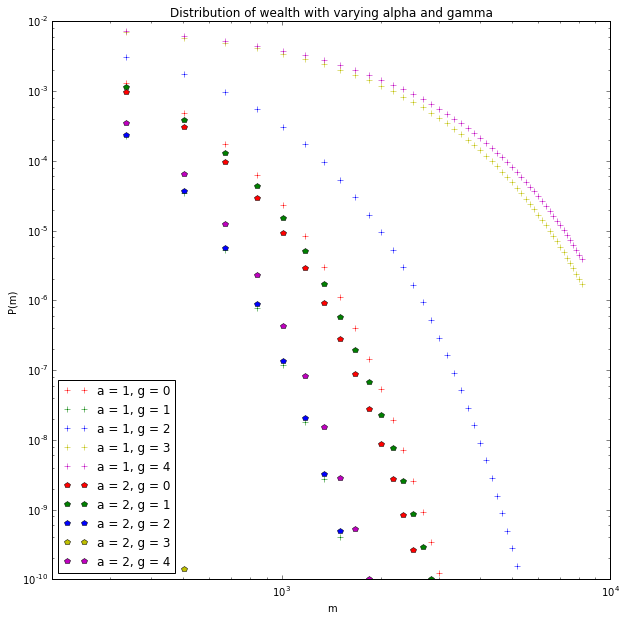
\includegraphics[height = 5.5cm]{Pareto_Distribution_Blown_Up.png}
		\caption{A zoomed in picture of the Pareto Distribution}
	\end{subfigure}
	\caption{The Pareto Distributions of our nearest neighbor and past transactions model. These behaviors match that of Goswami and Sen\cite{goswami}.}
	\label{Pareto}
\end{figure*}


\section{Discussion}
\subsection{Conservation of Money Numerical Precision} \label{conservation}
Based on how we defined the nature of these transactions, the total amount of money in the system should be conserved since proportions of the total money are being exchanged in each transaction. 

We ran a few scripts to determine if this was true and the results were troubling. Figure \ref{shit} shows that for the same simulation, the total money in the system is not being conserved and in different ways for the different simulations. The causes for this stem from our previous issues with numerical precision. Even with rounding all of our money values to 2 decimal places, rounding the random numbers to 2 places, and being careful to truncate our decimals at the correct values, Python has a systematic error with random number generation and lack of numerical precision. As a result, some randomly generated numbers can lead to jumps in the total amount of money in the system. Granted, they are negligible, but still present. The small magnitude of the variation allows us to assume that money is conserved throughout a simulation. Future work could be done to alleviate the issue of loss of numerical precision within our model in order to preserve "true" conservation. 

\begin{figure}[!ht]
	\centering
	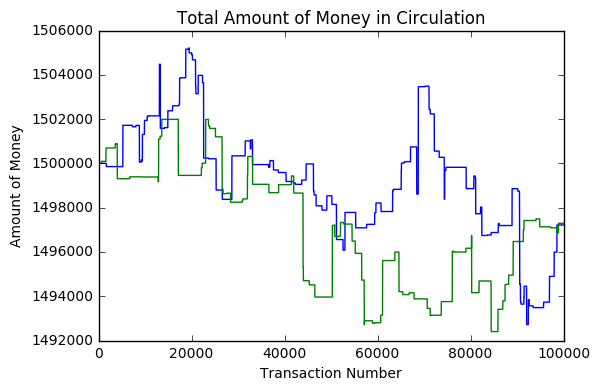
\includegraphics[height=4cm]{money_not_conserved.png}
	\caption{Plot of total money in a society. The same instance was modeled (N=1500, starting money=\$ 1000, transactions=$10^7$), and the blue and green lines show the respective results for total money in the system versus transaction number.}
	\label{shit}
\end{figure}

\subsection{Future Work}
Our simple model can be greatly expanded to model the messier and more complex real world.

A huge component would be implementing a system of taxation. We can do a simple sales tax model by taking away a percentage of money exchanged during each transaction and transferring it to a 3rd party that acts as our government. Another way of \sout{stealing} taking away this money would be to take a percentage of money that each agent already has after a set amount of iterations. This government can subsequently redistribute this money among the population. One would predict that the income distribution would be more even assuming the society doesn't collapse.

Another additional implementation is to remove the assumption that wealth is conserved. Real world economies prosper or collapse, and an individual's wealth changes based on this. Accounting for this would make for a more realistic macroscopic simulation. 

We could also include some mechanism where when individuals save money, they can earn interest on that money up until their next transaction. This would stem from the lack of conservation of money because we would be introducing new money into the system. This is more along the lines of real world situations and would be interesting to model.

Regardless of our decisions for future work, more sophisticated computational machines would be needed to handle the amount of floating point operations required for thorough analysis such as credit cards, taxation, saving interest, debt, etc. since our feeble laptop computers operate in a range where these types of models for large scale simulations could take hours. Improved equipment and implementation of more efficient languages (C++) could allow us to investigate more complex simulations and perhaps conduct new research into Econophysics.

\section{Conclusions}
We were able to use Monte Carlo methods of random number generation to simulate financial transactions for base scenarios including exchange of goods and services and savings. Using Householder's algorithm, we were also able to use random number generation to compare the likelihood of events for probability dependent transactions such as the nearest neighbor and previous interaction scenarios. Our results match the results made by the literature and we provided some possible considerations for future work to be done in Econophysics with similar modeling techniques.

Supplementary figures can be found with all working codes in our Github repository \cite{github}. 

\begin{thebibliography}{9}
	
	\bibitem{wikipedia} Econophysics. Wikipedia. \url{https://en.wikipedia.org/wiki/Econophysics}.
	
	\bibitem{pareto} Pareto, Vilfredo. \textit{Course on Political Economy}. \url{http://www.institutcoppet.org/2012/05/08/cours-deconomie-politique-1896-de-vilfredo-pareto}. 1896.
	
	\bibitem{patriarca} Patriarca, Marco, et al. \textit{Gibbs versus non-Gibbs distributions in money dynamics}. \url{http://www.sciencedirect.com/science/article/pii/S0378437104004327}. Physica A. Volume 340, Issues 1–3, 1 September 2004, Pages 334–339.
	
	\bibitem{goswami} Goswami, Sanchari. Sen, Parongama. \textit{Agent based models for wealth distribution with preference in interaction}. \url{http://www.sciencedirect.com/science/article/pii/S0378437114006967}. Physica A. Volume 415, 1 December 2014, Pages 514–524.
	
	\bibitem{morten} Hjorth-Jensen, Morten. Github for PHY480. \url{https://github.com/CompPhysics/ComputationalPhysicsMSU}.
	
	\bibitem{github} Github Repository for All Files. \url{https://github.com/nathawkins/PHY480MSU/tree/master/project4}.
	
\end{thebibliography}


\end{document}